\section{Исследовательская часть}

\subsection{Технические характеристики}

Технические характеристики устройства, на котором выполнялся замерный эксперимент:
\begin{itemize}[label*=---]
	\item операционная система Windows 11;
	\item память 16 ГБ;
	\item процессор 3,6 ГГц 6-ядерный процессор AMD Ryzen 5000 series 5.
\end{itemize}

Замеры проводились на ноутбуке, включенном в сеть электропитания. 
Во время тестирования ноутбук был нагружен только интегрированной средой разработки и непосредственно выполняемой программой.

\subsection{Пример работы программы}

На рисунке \ref{fig:example} представлен пример работы программы. 

\begin{figure}
	\centering
	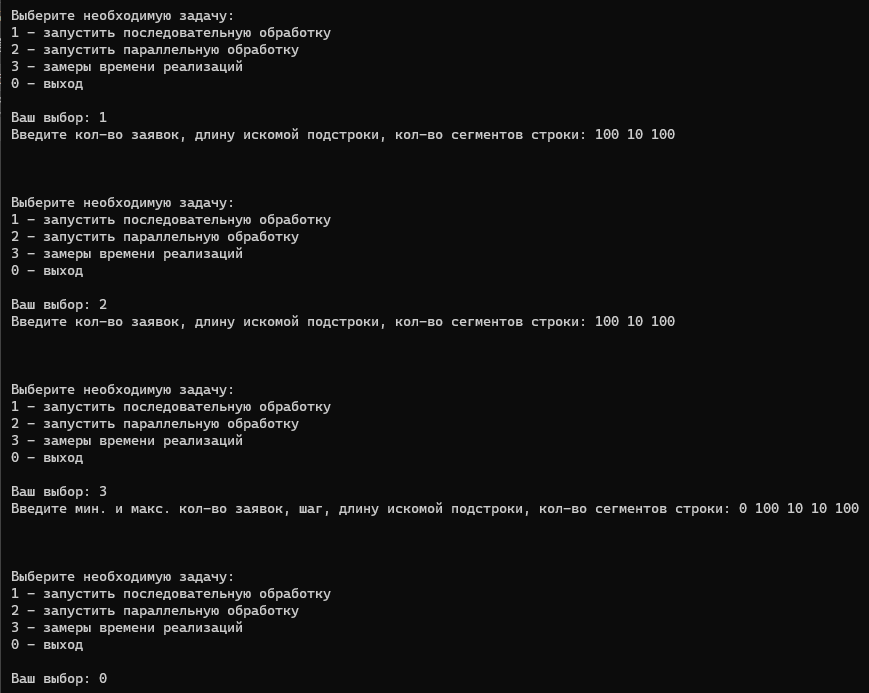
\includegraphics[width=1\linewidth]{images/example}
	\caption{Пример работы программы}
	\label{fig:example}
\end{figure}

ПО не выводит сообщения в консоль, но пишет их в лог.
На рисунке~\ref{fig:log_png} приведен его пример.
\begin{figure}
	\centering
	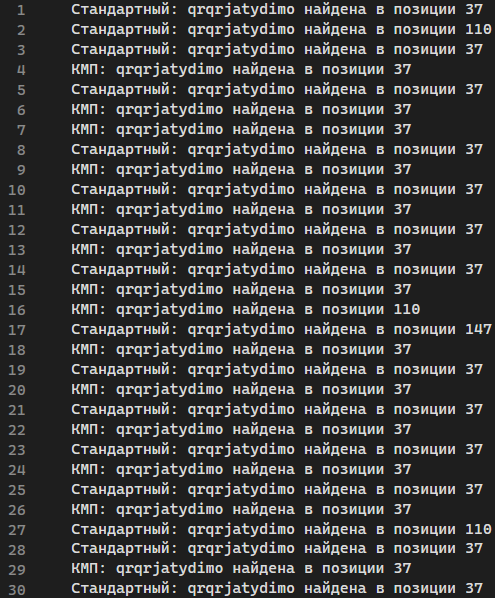
\includegraphics[width=0.7\linewidth]{images/log.png}
	\caption{Пример лога программы}
	\label{fig:log_png}
\end{figure}


\newpage

\subsection{Время выполнения реализованных алгоритмов}
Замер времени проводился с помощью библиотеки $chrono$~\cite{chrono}, в частности --- с помощью структуры $steady\_clock$~\cite{steady}.

Результаты измерений времени работы алгоритмов приведены на рисунке~\ref{fig:results}.
\begin{figure}
	\centering
	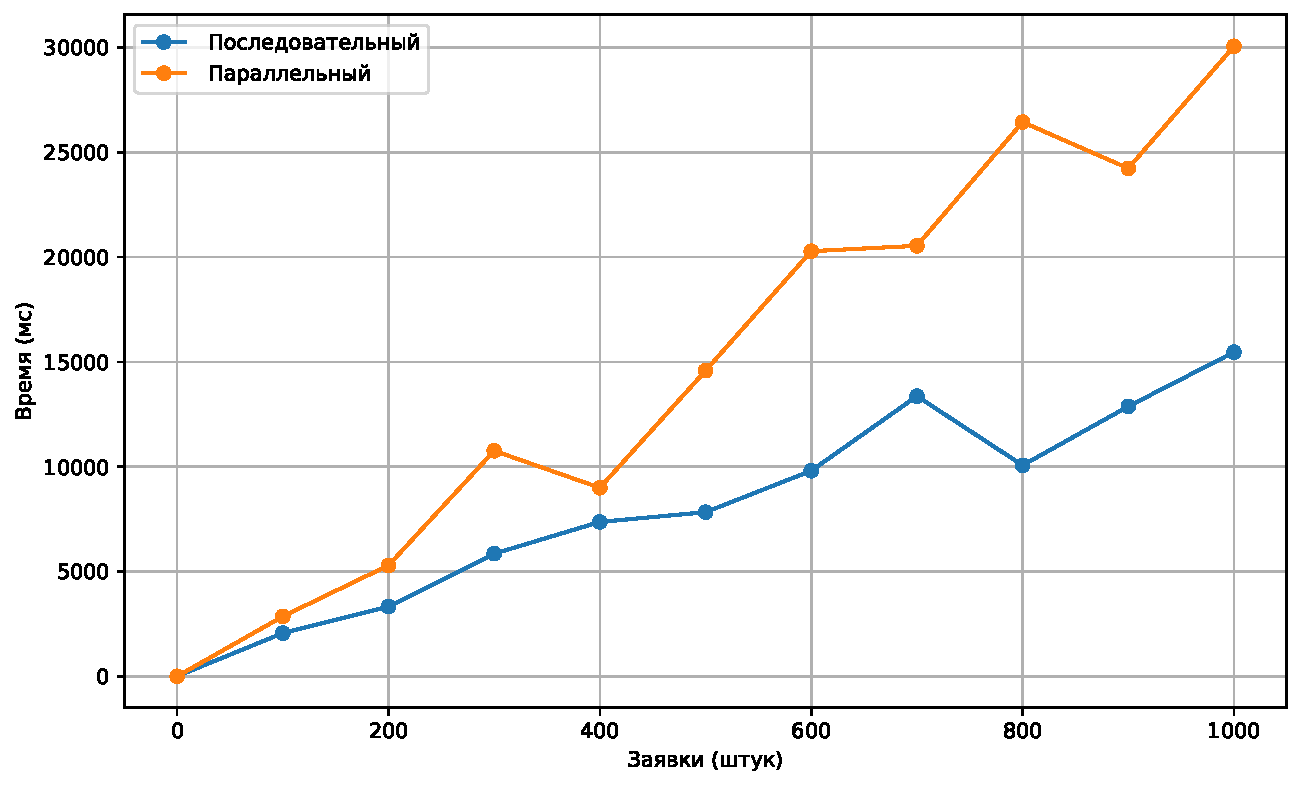
\includegraphics[width=1\linewidth]{../src/lab_05/time}
	\caption{Время выполнения алгоритмов}
	\label{fig:results}
\end{figure}

Время работы параллельной реализации конвейера во всех случаях больше его последовательной вариации.

\subsection*{Вывод}
Во всех случаях последовательная реализация конвейера выигрывает по времени у параллельной.
Происходит это из-за того, что время, которое тратится на управление потоками, не перекрывает <<выигрышь>> во времени, который достигается за счет одновременной обработки данных.
Как следствие --- последовательная реализация конвейера работает быстрее.
